% Οι άνθρωποι γνωρίζουν τα γινόμενα.
% Τα μέλλοντα γνωρίζουν οι θεοί,
\dictum[C. P. Kavafy]{Men know the material past, future deeds are
  known by gods}

\begin{summary}
\item FluiDB is well suited for join-heavy star schemata so we
  evaluated using the SSB-TPC-H benchmark.
\item Our evaluation shows that FluiDB is able to plan around the
  space constraints and come up with plans that materialize
  intermediate results that are useful for future queries.
\item FluiDB is generally faster than the baseline due to caching but
  at times may be slower in individual queries when it receives
  ``unexpected'' queries.
\item FluiDB generally performs better when allowed larger memory
  budgets but this speedup is based on heuristic assumptions that
  sometimes break in interesting ways.
\end{summary}

We based our evaluation on the Star Schema Benchmark (SSB)
\cite{barataOverviewDecisionSupport2015} which is a variation of
TPC-H. Like TPC-H it models the data warehouse of a wholesale
supplier.

As the name suggests, these queries query a star schema. The star
schema is derived from the TPC-H schema (figure \ref{fig:tpch_schema})
by merging the \sql{linenumber}, \sql{orders} and
\sql{partsupp} and completely dropped tables \sql{nation} and
\sql{region} tables as shown in figure \ref{fig:ssb_tpch_schema}.

\begin{figure}[p]
\begin{tikzdiagram}
  \tikzset{tbl/.style={draw,rectangle,minimum height=2cm,minimum width=2cm}};
  \node[tbl] (lo) {lineorder};
  \node[tbl] (p) [above left = of lo] {part};
  \node[tbl] (c) [above right = of lo] {customer};
  \node[tbl] (s) [below right = of lo] {supplier};
  \node[tbl] (d) [below left = of lo] {date};
  \draw [-stealth] (c) -- (lo);
  \draw [-stealth] (p) -- (lo);
  \draw [-stealth] (s) -- (lo);
  \draw [-stealth] (d) -- (lo);
\end{tikzdiagram}
\caption{\label{fig:ssb_tpch_schema}The foreign key links in a SSB-TPC-H}
\end{figure}


\begin{figure}[p]
\begin{tikzdiagram}
  \tikzset{tbl/.style={draw,rectangle,minimum height=2cm,minimum width=2cm}};
  \tikzset{arr/.style={-stealth}};
  \node[tbl]                     (r) {region};
  \node[tbl, right=of r]         (n) {nation};
  \node[tbl, above right = of n] (c) {customer};
  \node[tbl, right = of n] (s) {supplier};
  \node[tbl, right = of c]         (o) {orders};
  \node[tbl, right=of s]         (ps) {partsupp};
  \node[tbl, below left = of ps] (p) {part};
  \node[tbl, right= of ps]        (l) {lineitem};
  % Connection
  \path [arr]
  (r) edge (n)
  (n) edge (c)
  (c) edge (o)
  (o) edge (l)
  (n) edge (s)
  (s) edge (ps)
  (ps) edge (l)
  (p) edge (ps);
\end{tikzdiagram}
\caption{\label{fig:tpch_schema}The foreign key links in a traditional TPC-H schema}
\end{figure}


The particular queries contained in the workload are presented in
listing \ref{lst:ssb_sql} in the appendix (\ref{chapter:appendix}).

We generated a workload where queries were compiled and planned one by
one in a loop and were run over a database of data generated with
a modified version of the TPC-H dbgen
\cite{perivolaropoulosFakedrakeSsbdbgen2021a} with scaling of size 1,
meaning that the total primary data totals around 1GB in CSV format. The
exact size of the data generated after formatting them to the format
required by FluiDB (described in chapter \ref{chapter:execution_engine}) are

\begin{minted}[]{sh}
$ du -sh *.dat
4.1M    customer.dat
256K    date.dat
757M    lineorder.dat
31M     part.dat
268K    supplier.dat
\end{minted}

Which makes a total of approximately 200k pages of size 4KB.

The lowest budget within which FluiDB was able to plan all 13 queries
of SSB-TPC-H was 2300k pages.

In our experiment, we use page IO as a proxy for performance, despite
the fact that FluiDB is an in-memory database. We think that this is a
reasonable experimental approach because, as FluiDB leans heavily on
code generation, it is unlikely that the actual instruction retiring
will have a major impact on the performance. Instead, the performance
cost is dominated by page IO that will certainly cause cache misses at
the LLC. Another thing to note is that FluiDB generates code that
focuses on performance and not on compilation time, making heavy use
of metaprogramming like \cpp{constexpr} and temlpates.  This makes for
βfairly slow compilation times. There are ways to speed up compilation
time like using pre-compiling header files
\cite{PrecompiledHeadersPCH} and fine-tuning the compiler optimization
passes. These techniques are beyond the scope of this work, FluiDB is
focused on analytics workloads that do not include sub-second queries.

\newcommand{\ioperfdescr}{The total page read/writes for
  each query of SSB TPC-H. The baseline is the query being
  run by FluiDB directly without any materialized n-nodes. The workload
  bars represent the cost of each query in a workload being
  accumulated into the same QDAG.}
\begin{figure}[p]
\centering
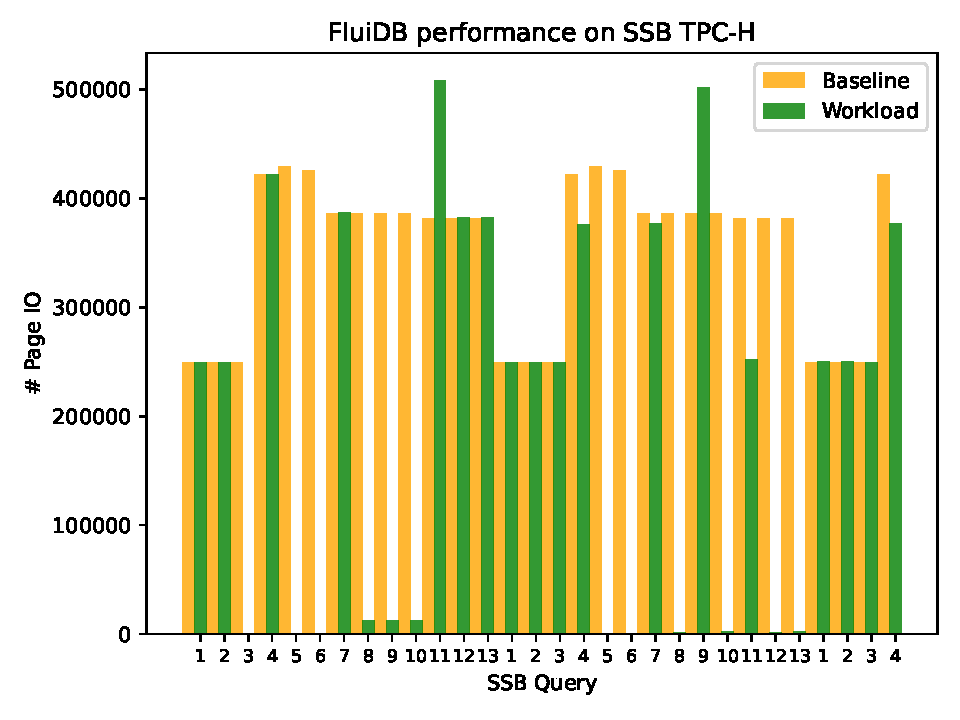
\includegraphics[width=.9\linewidth]{./plans/io_perf_23000.pdf}
\caption{\label{fig:min_budget_plot} \ioperfdescr The budget allowed
  for this is the minimum budget within which FluiDB can run each
  individual query (2300K pages).}
\end{figure}

Figure \ref{fig:min_budget_plot} demonstrates that FluiDB running a
workload versus running individual queries causes significant speedups
even in constrained budgets. In some cases, however, the garbage
collector is forced to delete tables that need to be recreated later
in the workload causing FluiDB to be sporadically less performant than
the base case.

For a larger budget, the FluiDB is able to store more useful
intermediate results as demonstrated in figure \ref{fig:large_budget_plot}

\begin{figure}[p]
\centering
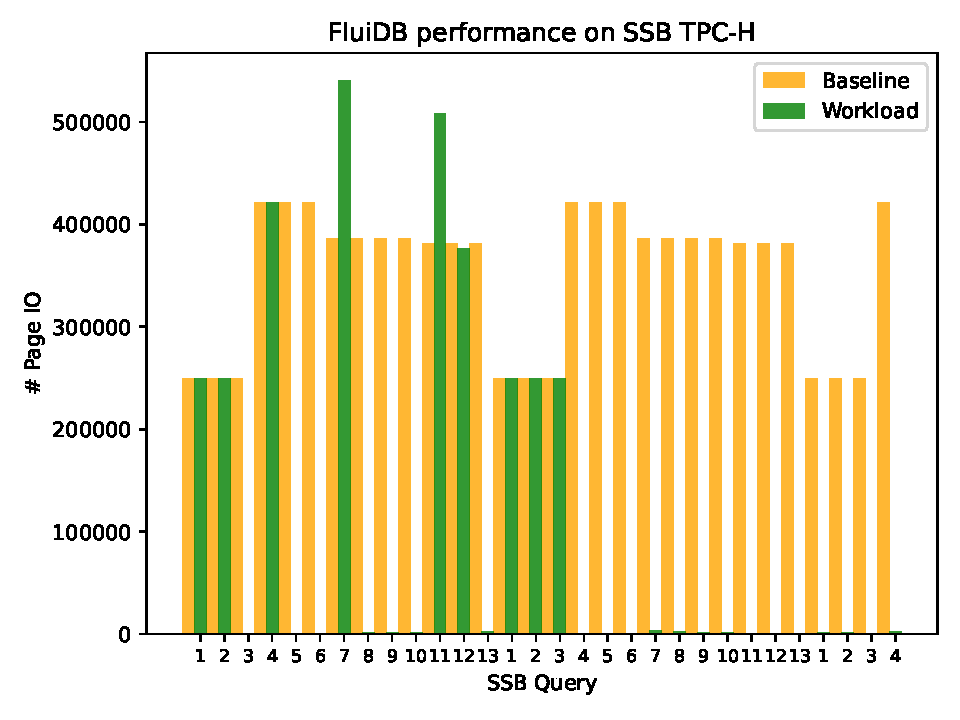
\includegraphics[width=.9\linewidth]{./plans/io_perf_61000.pdf}

\caption{\label{fig:large_budget_plot} \ioperfdescr The budget
  allowed for this is about triple the minimum budget within which
  FluiDB can run each individual query (6100K pages). A badly timed GC
  run causes some individual queries to be slower than their
  counterparts from a workload being run in a tight budget (figure
  \ref{fig:min_budget_plot}.}
\end{figure}

An interesting point here is the plan for evaluating query 7 is more
expensive in the workload run under laxer budgetary constraints. This
may seem strange but it is an example demonstrative of the
fundamental operation of FluiDB.

The top level explanation is that the high-budget plan needs to
evaluate \(\mathit{lineorder}\) via the reverse trigger of a join as
it was deleted during the evaluation of query 6. Mysteriously, during the
strict-budget planning the \(\mathit{lineorder}\) relation is readily
available during the planning of query 7! The key lies slightly earlier in
the workload (see listing \ref{fig:reverse_operations}).

FluiDB materializes in query 4 the join

\[
Q_{36} := \mathit{supplier} \Join_{\mathit{lo\_suppkey} = \mathit{s\_suppkey}} \mathit{lineorder}
\]

and the corresponding antijoins \(Q_{35}\) and \(Q_{37}\) making the node
\(\mathit{lineorder}\) deletable. However, when running the workload
under strict budgetary constraints, it is forced to garbage collect
shortly after materializing said join at a moment while both \(Q\) and
\(\mathit{lineorder}\) are protected (see section \ref{sec:gc} on
garbage collection). Therefore, FluiDB is forced to delete both
\(Q_{35}\) and \(Q_{37}\). Making \(\mathit{lineorder}\) non-deletable
when planning for query 4 finishes.

\begin{code}
\begin{minted}[escapeinside=||,mathescape=true]{trace-lexer.py:TraceLexer -x}
# Query 4
Query |\(s \gamma \pi \sigma (\mathit{supplier} \Join \mathit{lineorder} \Join \mathit{date} \Join \mathit{part})\)| {
  # There is enough space to keep both and the complements
  |\(Q_{36}, Q_{35}, Q_{37}\)| := Materialize[|\(\mathit{supplier} \Join \mathit{lineorder}, \mathit{supplier} \cancel\ltimes \mathit{lineorder}, \mathit{supplier} \cancel\rtimes \mathit{lineorder}\)|]
  |\(Q_{41}, Q_{40}, Q_{42}\)| := Materialize[|\(Q_{36} \Join \mathit{date}, Q_{36} \cancel\ltimes \mathit{date}, Q_{36} \cancel\rtimes \mathit{date}\)|]
  |\(Q_{46}, Q_{45}, Q_{47}\)| := Materialize[|\(Q_{41} \Join \mathit{part}, Q_{41} \cancel\ltimes \mathit{part}, Q_{41} \cancel\rtimes \mathit{part}\)|]
  |\(Q_{50}\)| := Materialize[|\(\sigma Q_{46}\)|]
  |\(Q_{90}\)| := Materialize[|\(\gamma \pi Q_{50}\)|]
  |\(Q_{91}\)| := Materialize[|\(s Q_{90}\)|]
}

# Query 5
Query |\(s \gamma \pi \sigma (\mathit{supplier} \Join \mathit{lineorder} \Join \mathit{date} \Join \mathit{part})\)| {
  |\(Q_{92}\)| := Materialize[|\(\sigma Q_{46}\)|]
  |\(Q_{118}\)| := Materialize[|\(\gamma \pi Q_{92}\)|]
  |\(Q_{119}\)| := Materialize[|\(s Q_{118}\)|]
}

# Query 6
Query |\(s \gamma \pi \sigma (\mathit{supplier} \Join \mathit{lineorder} \Join \mathit{date} \Join \mathit{part}))\)| {
  # FluiDB decides delete lineorder since it has the complements
  GC { Delete[|\(\ldots, \mathit{lineorder}, \ldots \)|] }
  |\(Q_{120}\)| := Materialize[|\(\sigma Q_{46}\)|]
  |\(Q_{146}\)| := Materialize[|\(\gamma \pi Q_{120}\)|]
  |\(Q_{147}\)| := Materialize[|\(s Q_{146}\)|]
}

# Query 7
Query |\(s \gamma \pi \sigma (\mathit{customer} \Join \mathit{date} \Join \mathit{lineorder} \Join \mathit{supplier})\)| {
  # Ooops... this would be avoided if we hadn't deleted lineorder.
  |\(\mathit{lineorder}\)| := Materialize[|\(\bar\pi Q_{36} \cup Q_{37}\)|]
  |\(\mathit{date}\)| := Materialize[|\(\bar\pi Q_{41} \cup Q_{42}\)|]
  GC { Delete[|\( \ldots \)|] }
  |\(Q_{149}, Q_{148}, Q_{150}\)| := Materialize[|\(\mathit{date} \Join \mathit{lineorder}, \mathit{date} \cancel\ltimes \mathit{lineorder}, \mathit{date} \cancel\rtimes \mathit{lineorder}\)|]
  GC { Delete[|\( \ldots \)|] }
  |\(Q_{154}, Q_{153}, Q_{155}\)| := Materialize[|\(\mathit{customer} \Join Q_{149}, \mathit{customer} \cancel\ltimes Q_{149}, \mathit{customer} \cancel\rtimes Q_{149}\)|]
  GC { Delete[|\( \ldots \)|] }
  |\(Q_{165}\)| := Materialize[|\(\sigma Q_{154}\)|]
  |\(Q_{182}, Q_{181}, Q_{183}\)| := Materialize[|\(Q_{165} \Join \mathit{supplier}, Q_{165} \cancel\ltimes \mathit{supplier}, Q_{165} \cancel\rtimes \mathit{supplier}\)|]
  GC { Delete[|\( \ldots \)|] }
  |\(Q_{163}\)| := Materialize[|\(\sigma Q_{182}\)|]
  |\(Q_{203}\)| := Materialize[|\(\gamma \pi Q_{163}\)|]
  |\(Q_{204}\)| := Materialize[|\(s Q_{203}\)|]
}

\end{minted}
  \caption{\label{fig:reverse_operations}Abbreviated version of the
    plans of queries 4 to 7 of SSB TPC-H. This demonstrates how an
    unfortunately timed GC can cause cause FluiDB to make some bad decisions}

\end{code}


On the other hand, with laxer budgetary constraints, no garbage
collection is triggered during query 4. The next garbage
collection is triggered during query 6, at a moment when
\(\mathit{lineorder}\) is deletable, unprotected, and a prime
candidate for deletion based on the GC heuristics.

Alas, when query 7 requires \(\mathit{lineorder}\) for its plan,
FluiDB needs to reconstruct it in the case of lax budgetary
constraints but not in the case of strict constraints.

This example of FluiDB being forced to locally produce more expensive
plans is an effect of FluiDB being more opportunistic, the lower the
available budget is, and more adventurous when operating with high
budgets. When FluiDB is frugal, it is generally prone to miss
opportunities to share computation between queries. There are times
however that this frugality saves it from bad heuristic-based decisions
that it is allowed to make otherwise.

FluiDB aspires to deal with the entire workload as if it were planning
a single query. While any decision during the planning of a single
query can be scrapped in the backtracking process, FluiDB is
tragically forced to commit to whatever adventurous or conservative
decisions it makes at the end of every planning iteration, doomed to
pay dearly for every misstep but to reap the rewards of every
insightful choice.

Interestingly, this problem goes away when we run with a budget of
3500k pages (figure \ref{fig:extra_large_budget_plot}) as the GC run
is delayed to a time when other relations are better candidates for
deletion than \(\mathit{lineorder}\). A carefully designed set of
heuristics for the GC should avoid this problem in most cases.

\begin{figure}[p]
\centering
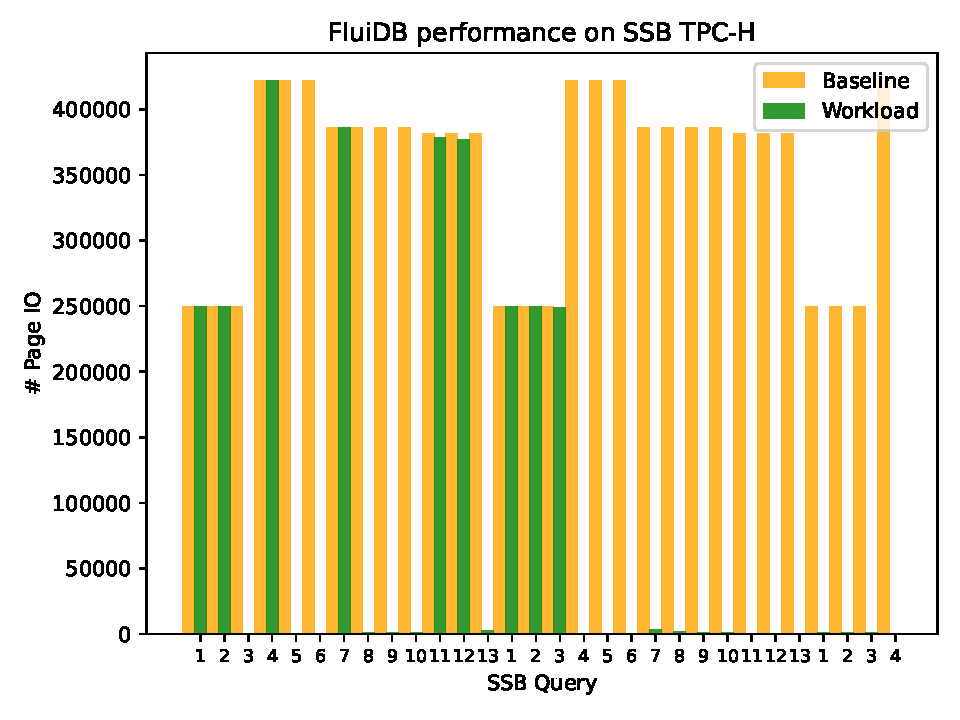
\includegraphics[width=.9\linewidth]{./plans/io_perf_65000.pdf}

\caption{\label{fig:extra_large_budget_plot}
\ioperfdescr. The budget
  allowed for this is about triple the minimum budget within which
  FluiDB can run each individual query (6500K pages).}
\end{figure}

\section{A note on size estimation}
\label{sec:size_estimation_problems}
The size of the budget may seem fairly excessive for the size required
for the primary tables. To understand why that is, we need to look at
the largest n-nodes in the QDAG:

\begin{center}
\begin{tabular}{rl}
Pages & Expr\\
\hline
188000 & \(lineorder\)\\
547100 & \(customer \Join (date \Join lineorder)\)\\
376200 & \(\sigma ((customer \Join (date \Join lineorder)) \Join supplier)\)\\
376200 & \(\sigma ((date \Join lineorder)) \Join supplier)\)\\
273600 & \(\sigma (customer \Join (date \Join lineorder))\)\\
188100 & \(\sigma ((\sigma (customer \Join (date \Join lineorder))) \Join supplier)\)\\
\end{tabular}
\end{center}

From looking at those n-nodes it seems that a sufficiently advanced
garbage collector should be able to support plans that materialize the
n-nodes in about half the budget as FluiDB should have been able to plan
the query needing around double the pages required to store the largest equijoin
which for us is \(customer\) date \(lineorder\).

The main issue, however, as it is with many query processing systems
\cite{leisHowGoodAre2015}, is the cardinality estimator which assumes
that in a natural join there are no foreign key lookup failures, that
is, that all natural joins are extension joins. Therefore

\[
\lvert \sigma _{p(customer)} (customer \Join (date \Join lineorder)) \rvert = \lvert (\sigma _{p(customer)} customer \Join (date \Join lineorder)) \rvert
\]


This causes FluiDB to vastly overestimate the size of plans that have
selections pushed down, making these plans disproportionately
unappealing.


\section{Conclusion}

FluiDB is a complex database system built from scratch focused on
a specific idea: making optimal use of the storage budget by fully
adapting the data layout to the workload. While FluiDB itself it is
far from stable enough system to be used in a production setting, the
results presented in this chapter demonstrate that it is an idea worth
considering to incorporate in the design of a commercial database system.
